\documentclass{article} % For LaTeX2e
\usepackage{iclr2024_conference,times}

\usepackage[utf8]{inputenc} % allow utf-8 input
\usepackage[T1]{fontenc}    % use 8-bit T1 fonts
\usepackage{hyperref}       % hyperlinks
\usepackage{url}            % simple URL typesetting
\usepackage{booktabs}       % professional-quality tables
\usepackage{amsfonts}       % blackboard math symbols
\usepackage{nicefrac}       % compact symbols for 1/2, etc.
\usepackage{microtype}      % microtypography
\usepackage{titletoc}

\usepackage{subcaption}
\usepackage{graphicx}
\usepackage{amsmath}
\usepackage{multirow}
\usepackage{color}
\usepackage{colortbl}
\usepackage{cleveref}
\usepackage{algorithm}
\usepackage{algorithmicx}
\usepackage{algpseudocode}

\DeclareMathOperator*{\argmin}{arg\,min}
\DeclareMathOperator*{\argmax}{arg\,max}

\graphicspath{{../}} % To reference your generated figures, see below.
\begin{filecontents}{references.bib}

@book{goodfellow2016deep,
  title={Deep learning},
  author={Goodfellow, Ian and Bengio, Yoshua and Courville, Aaron and Bengio, Yoshua},
  volume={1},
  year={2016},
  publisher={MIT Press}
}

@article{vaswani2017attention,
  title={Attention is all you need},
  author={Vaswani, Ashish and Shazeer, Noam and Parmar, Niki and Uszkoreit, Jakob and Jones, Llion and Gomez, Aidan N and Kaiser, {\L}ukasz and Polosukhin, Illia},
  journal={Advances in neural information processing systems},
  volume={30},
  year={2017}
}

@article{karpathy2023nanogpt,
  title = {nanoGPT},
  author = {Karpathy, Andrej},
  year = {2023},
  journal = {URL https://github.com/karpathy/nanoGPT/tree/master},
  note = {GitHub repository}
}

@article{kingma2014adam,
  title={Adam: A method for stochastic optimization},
  author={Kingma, Diederik P and Ba, Jimmy},
  journal={arXiv preprint arXiv:1412.6980},
  year={2014}
}

@article{ba2016layer,
  title={Layer normalization},
  author={Ba, Jimmy Lei and Kiros, Jamie Ryan and Hinton, Geoffrey E},
  journal={arXiv preprint arXiv:1607.06450},
  year={2016}
}

@article{loshchilov2017adamw,
  title={Decoupled weight decay regularization},
  author={Loshchilov, Ilya and Hutter, Frank},
  journal={arXiv preprint arXiv:1711.05101},
  year={2017}
}

@article{radford2019language,
  title={Language Models are Unsupervised Multitask Learners},
  author={Radford, Alec and Wu, Jeff and Child, Rewon and Luan, David and Amodei, Dario and Sutskever, Ilya},
  year={2019}
}

@article{bahdanau2014neural,
  title={Neural machine translation by jointly learning to align and translate},
  author={Bahdanau, Dzmitry and Cho, Kyunghyun and Bengio, Yoshua},
  journal={arXiv preprint arXiv:1409.0473},
  year={2014}
}

@article{paszke2019pytorch,
  title={Pytorch: An imperative style, high-performance deep learning library},
  author={Paszke, Adam and Gross, Sam and Massa, Francisco and Lerer, Adam and Bradbury, James and Chanan, Gregory and Killeen, Trevor and Lin, Zeming and Gimelshein, Natalia and Antiga, Luca and others},
  journal={Advances in neural information processing systems},
  volume={32},
  year={2019}
}

@misc{gpt4,
  title={GPT-4 Technical Report}, 
  author={OpenAI},
  year={2024},
  eprint={2303.08774},
  archivePrefix={arXiv},
  primaryClass={cs.CL},
  url={https://arxiv.org/abs/2303.08774}, 
}

@Article{Zeiler2013VisualizingAU,
 author = {Matthew D. Zeiler and R. Fergus},
 booktitle = {European Conference on Computer Vision},
 journal = {ArXiv},
 title = {Visualizing and Understanding Convolutional Networks},
 volume = {abs/1311.2901},
 year = {2013}
}


@Book{Ribeiro2016WhySI,
 author = {Marco Tulio Ribeiro and Sameer Singh and Carlos Guestrin},
 booktitle = {North American Chapter of the Association for Computational Linguistics},
 journal = {Proceedings of the 22nd ACM SIGKDD International Conference on Knowledge Discovery and Data Mining},
 title = {“Why Should I Trust You?”: Explaining the Predictions of Any Classifier},
 year = {2016}
}


@Article{Chen2019RobustAR,
 author = {Jiefeng Chen and Xi Wu and Vaibhav Rastogi and Yingyu Liang and S. Jha},
 booktitle = {Neural Information Processing Systems},
 journal = {ArXiv},
 title = {Robust Attribution Regularization},
 volume = {abs/1905.09957},
 year = {2019}
}


@Article{Cunningham2023SparseAF,
 author = {Hoagy Cunningham and Aidan Ewart and Logan Riggs and R. Huben and Lee Sharkey},
 booktitle = {International Conference on Learning Representations},
 journal = {ArXiv},
 title = {Sparse Autoencoders Find Highly Interpretable Features in Language Models},
 volume = {abs/2309.08600},
 year = {2023}
}


@Article{Bengio2007LearningDA,
 author = {Yoshua Bengio},
 booktitle = {Found. Trends Mach. Learn.},
 journal = {Found. Trends Mach. Learn.},
 pages = {1-127},
 title = {Learning Deep Architectures for AI},
 volume = {2},
 year = {2007}
}


@Article{Dunefsky2024TranscodersFI,
 author = {Jacob Dunefsky and Philippe Chlenski and Neel Nanda},
 booktitle = {arXiv.org},
 journal = {ArXiv},
 title = {Transcoders Find Interpretable LLM Feature Circuits},
 volume = {abs/2406.11944},
 year = {2024}
}

@Article{Makelov2024TowardsPE,
 author = {Aleksandar Makelov and Georg Lange and Neel Nanda},
 booktitle = {arXiv.org},
 journal = {ArXiv},
 title = {Towards Principled Evaluations of Sparse Autoencoders for Interpretability and Control},
 volume = {abs/2405.08366},
 year = {2024}
}


@Article{Chen2020ASF,
 author = {Ting Chen and Simon Kornblith and Mohammad Norouzi and Geoffrey E. Hinton},
 booktitle = {International Conference on Machine Learning},
 journal = {ArXiv},
 title = {A Simple Framework for Contrastive Learning of Visual Representations},
 volume = {abs/2002.05709},
 year = {2020}
}


@Article{Cao2021EditingFK,
 author = {Nicola De Cao and Wilker Aziz and Ivan Titov},
 booktitle = {Conference on Empirical Methods in Natural Language Processing},
 pages = {6491-6506},
 title = {Editing Factual Knowledge in Language Models},
 year = {2021}
}


@Article{Paulo2024AutomaticallyIM,
 author = {Gonccalo Paulo and Alex Troy Mallen and Caden Juang and Nora Belrose},
 booktitle = {arXiv.org},
 journal = {ArXiv},
 title = {Automatically Interpreting Millions of Features in Large Language Models},
 volume = {abs/2410.13928},
 year = {2024}
}


@Article{Hjelm2018LearningDR,
 author = {R. Devon Hjelm and A. Fedorov and Samuel Lavoie-Marchildon and Karan Grewal and Adam Trischler and Yoshua Bengio},
 booktitle = {International Conference on Learning Representations},
 journal = {ArXiv},
 title = {Learning deep representations by mutual information estimation and maximization},
 volume = {abs/1808.06670},
 year = {2018}
}


@Article{Cao2021EditingFK,
 author = {Nicola De Cao and Wilker Aziz and Ivan Titov},
 booktitle = {Conference on Empirical Methods in Natural Language Processing},
 pages = {6491-6506},
 title = {Editing Factual Knowledge in Language Models},
 year = {2021}
}


@Article{Arik2019AttentionBasedPL,
 author = {Sercan Ö. Arik and Tomas Pfister},
 booktitle = {arXiv.org},
 journal = {ArXiv},
 title = {Attention-Based Prototypical Learning Towards Interpretable, Confident and Robust Deep Neural Networks},
 volume = {abs/1902.06292},
 year = {2019}
}


@Article{Elhage2022ToyMO,
 author = {Nelson Elhage and Tristan Hume and Catherine Olsson and Nicholas Schiefer and T. Henighan and Shauna Kravec and Zac Hatfield-Dodds and R. Lasenby and Dawn Drain and Carol Chen and R. Grosse and Sam McCandlish and Jared Kaplan and Dario Amodei and M. Wattenberg and C. Olah},
 booktitle = {arXiv.org},
 journal = {ArXiv},
 title = {Toy Models of Superposition},
 volume = {abs/2209.10652},
 year = {2022}
}


@Article{Bau2017NetworkDQ,
 author = {David Bau and Bolei Zhou and A. Khosla and A. Oliva and A. Torralba},
 booktitle = {Computer Vision and Pattern Recognition},
 journal = {2017 IEEE Conference on Computer Vision and Pattern Recognition (CVPR)},
 pages = {3319-3327},
 title = {Network Dissection: Quantifying Interpretability of Deep Visual Representations},
 year = {2017}
}

\end{filecontents}

\title{The Limits of Structural Approaches to Knowledge Separation: A Systematic Study of Hierarchical Sparse Autoencoders}

\author{LLM\\
Department of Computer Science\\
University of LLMs\\
}

\newcommand{\fix}{\marginpar{FIX}}
\newcommand{\new}{\marginpar{NEW}}

\begin{document}

\maketitle

\begin{abstract}
The ability to isolate and modify specific knowledge within large language models is crucial for maintaining and updating AI systems, yet achieving clean knowledge separation remains an unsolved challenge. While sparse autoencoders have shown promise for neural interpretation, we demonstrate fundamental limitations in structural approaches to knowledge disentanglement. Through systematic experimentation with the Gemma-2B model, we develop increasingly sophisticated architectures culminating in a novel contrastive hierarchical sparse autoencoder that combines dynamic feature grouping, attention-based assignment mechanisms, and multi-level orthogonality constraints. Despite implementing an optimized 8$\times$8 hierarchical structure with carefully tuned parameters ($\alpha_{L1}=0.4$, $\alpha_{L2}=0.2$) and InfoNCE contrastive loss (temperature=0.1), our approach fails to achieve effective knowledge separation, with unlearning scores remaining at 0.0 across all variants. Our detailed ablation study across six architectural iterations reveals that even sophisticated combinations of modern deep learning techniques cannot overcome these limitations, suggesting the need for fundamentally new approaches beyond structural organization for achieving selective knowledge modification in large language models.
\end{abstract}

\section{Introduction}
\label{sec:intro}

The ability to selectively modify knowledge within large language models (LLMs) is crucial for maintaining and updating AI systems, yet achieving reliable knowledge separation remains an unsolved challenge \cite{gpt4}. While LLMs have revolutionized natural language processing, their distributed representations make it difficult to isolate and modify specific knowledge components without affecting other capabilities \cite{goodfellow2016deep}. This challenge has significant implications for model maintenance, bias mitigation, and regulatory compliance, particularly as LLMs become increasingly integrated into critical applications.

Recent work has demonstrated that sparse autoencoders can extract interpretable features from language models \cite{Paulo2024AutomaticallyIM}, suggesting potential for knowledge separation. However, initial experiments with simple orthogonality constraints ($\alpha=0.1$) revealed fundamental limitations, with unlearning scores consistently at 0.0 despite achieving high reconstruction accuracy. The challenge stems from the inherently distributed nature of neural representations \cite{Elhage2022ToyMO}, where knowledge is encoded through complex patterns of activation across many neurons in ways that resist simple structural organization.

We systematically explore this limitation through six architectural iterations of increasing sophistication, focusing on layer 19 of the Gemma-2B model. Our progression begins with fixed orthogonality constraints ($\alpha=0.1$), advances through dynamic feature grouping (32-64 groups), and culminates in a novel contrastive hierarchical sparse autoencoder. This final architecture implements an 8$\times$8 hierarchical structure with attention-based group assignment (updated every 50 steps) and InfoNCE contrastive loss (temperature=0.1, weight=0.1), representing a significant advance in architectural complexity for knowledge separation.

Our main contributions are:
\begin{itemize}
    \item A systematic evaluation of increasingly sophisticated feature separation strategies, from basic orthogonal constraints through dynamic grouping to hierarchical organization, revealing fundamental limitations in structural approaches
    \item A novel hierarchical sparse autoencoder combining multi-level orthogonality constraints ($\alpha_{L1}=0.4$, $\alpha_{L2}=0.2$), attention-based group assignment, and contrastive learning
    \item Comprehensive ablation studies across six architectural variants demonstrating that even sophisticated combinations of modern deep learning techniques fail to achieve non-zero unlearning scores
    \item Critical insights into the limitations of purely structural approaches to knowledge separation, supported by detailed experimental results on the WMDP-bio dataset
\end{itemize}

Our experimental results reveal persistent limitations in current approaches to feature disentanglement. Despite implementing increasingly sophisticated architectures and carefully tuning parameters, unlearning scores remained at 0.0 across all variants. These findings suggest that achieving true knowledge separation may require fundamentally new approaches beyond structural organization, potentially focusing on semantic relationships or task-specific objectives. This work provides important negative results for the field while highlighting crucial questions about the nature of knowledge representation in large language models.

\section{Related Work}
\label{sec:related}
% Structure outline for Related Work section
% 1. Prior Work on Neural Network Interpretability
%    - Focus on methods analyzing internal representations
%    - Compare to our approach of using SAEs for feature separation
%    - Contrast with techniques like attribution methods and probing
%    - Key papers: [Goodfellow2016] for foundational concepts

% 2. Sparse Autoencoders and Knowledge Separation
%    - Review existing SAE architectures and their limitations
%    - Compare hierarchical organization approaches
%    - Contrast with our dynamic feature grouping method
%    - Key papers: [Vaswani2017] for attention mechanisms

% 3. Contrastive Learning in Feature Extraction
%    - Examine contrastive approaches in representation learning
%    - Compare with our InfoNCE-based feature separation
%    - Discuss limitations in knowledge disentanglement
%    - Key papers: [Kingma2014] for optimization insights

% 4. Knowledge Editing in Language Models
%    - Review current approaches to selective knowledge modification
%    - Compare unlearning methods and their effectiveness
%    - Contrast with our hierarchical feature separation
%    - Key papers: [Ba2016] for normalization techniques

% Note: All citations will use existing references.bib entries
% Focus on comparing/contrasting approaches rather than just describing
% Emphasize why some methods aren't applicable to our problem
% Lead into our novel contributions

Prior approaches to neural network interpretability can be broadly categorized by their assumptions about knowledge representation and modification. Attribution methods \cite{Zeiler2013VisualizingAU, Ribeiro2016WhySI} assume that model decisions can be explained through input feature importance, but unlike our approach, they cannot directly modify internal representations. Network dissection \cite{Bau2017NetworkDQ} assumes interpretable units exist within networks, successfully identifying them in CNNs, but this assumption breaks down in transformer architectures where our experiments show knowledge is more diffusely distributed.

Sparse autoencoders \cite{Bengio2007LearningDA, Cunningham2023SparseAF} share our goal of disentangling neural representations but differ in their approach to feature organization. While previous work focuses on identifying interpretable features through sparsity alone, our hierarchical architecture explicitly enforces structured relationships between feature groups. Recent evaluations \cite{Makelov2024TowardsPE} demonstrate that simple sparsity achieves interpretability but fails at selective modification - a limitation we attempted to overcome through contrastive learning and dynamic feature grouping, though ultimately encountering similar barriers.

The closest approaches to our work are transcoders \cite{Dunefsky2024TranscodersFI} and direct editing methods \cite{Cao2021EditingFK}, which also target knowledge modification in language models. Transcoders differ by learning mappings between model representations rather than attempting internal reorganization, while direct editing methods modify weights without attempting to understand feature organization. Our negative results with increasingly sophisticated structural approaches suggest these alternative paradigms may be more promising for achieving selective knowledge modification.

\section{Background}
\label{sec:background}

Recent work has demonstrated that transformer-based language models encode knowledge in complex distributed representations \cite{Elhage2022ToyMO}, making selective modification of specific concepts challenging. While sparse autoencoders have shown promise for neural interpretation \cite{Cunningham2023SparseAF}, achieving true knowledge separation remains difficult due to the inherent superposition of concepts across neurons \cite{Elhage2022ToyMO}. This challenge is particularly acute in large language models where selective unlearning capabilities are increasingly important for maintenance and updating.

Traditional approaches to feature disentanglement in neural networks have focused on structural constraints like orthogonality \cite{Bengio2007LearningDA} and sparsity \cite{Cunningham2023SparseAF}. However, these methods often fail to achieve clean knowledge separation in transformer architectures, where semantic concepts can be encoded across multiple attention heads and feed-forward layers \cite{vaswani2017attention}. Our work systematically explores the limitations of these approaches through increasingly sophisticated architectural variants.

\subsection{Problem Setting}
Let $\mathbf{x} \in \mathbb{R}^d$ represent activations from layer $l$ of a pre-trained language model $\mathcal{M}$. We aim to learn an encoder-decoder pair $(E,D)$ that maps these activations to a sparse, interpretable representation while preserving the model's computational capabilities. Formally, we seek functions:

\begin{align*}
E &: \mathbb{R}^d \rightarrow \mathbb{R}^n \\
D &: \mathbb{R}^n \rightarrow \mathbb{R}^d
\end{align*}

subject to three key constraints:

\begin{enumerate}
    \item \textbf{Reconstruction}: $\|D(E(\mathbf{x})) - \mathbf{x}\|_2 \leq \epsilon$
    \item \textbf{Sparsity}: $\|E(\mathbf{x})\|_1 \leq \lambda$
    \item \textbf{Knowledge Separation}: For any two semantic concepts $c_1, c_2$, their feature activations should be orthogonal: $\langle E(\mathbf{x}_{c_1}), E(\mathbf{x}_{c_2}) \rangle \approx 0$
\end{enumerate}

The encoder and decoder are implemented as single-layer neural networks:
\begin{align*}
E(\mathbf{x}) &= \text{ReLU}(\mathbf{W}_e\mathbf{x} + \mathbf{b}_e) \\
D(\mathbf{h}) &= \mathbf{W}_d\mathbf{h} + \mathbf{b}_d
\end{align*}

where $\mathbf{W}_e \in \mathbb{R}^{n \times d}$, $\mathbf{W}_d \in \mathbb{R}^{d \times n}$, and $\mathbf{b}_e, \mathbf{b}_d$ are bias terms. The ReLU activation ensures non-negative sparse features.

Our key assumption is that knowledge in language models can be separated through appropriate structural constraints on these representations. We test this hypothesis through six architectural variants with increasing sophistication, from basic orthogonality constraints to hierarchical feature organization with contrastive learning.

\section{Method}
\label{sec:method}

Building on the formalism from Section~\ref{sec:background}, we develop a hierarchical sparse autoencoder that attempts to separate knowledge through structured feature organization. Our approach extends the basic encoder-decoder framework with three key components: hierarchical grouping, dynamic assignment, and contrastive learning.

\subsection{Hierarchical Feature Organization}
Given encoded features $\mathbf{h} = E(\mathbf{x})$, we organize the $n$-dimensional representation space into a two-level hierarchy:

\begin{equation}
    \mathbf{h} = \bigcup_{i=1}^8 \bigcup_{j=1}^8 g_2^{i,j}, \quad g_2^{i,j} \subset g_1^i
\end{equation}

where $g_1^i$ represents one of 8 coarse-grained groups and $g_2^{i,j}$ represents one of 8 fine-grained subgroups within each $g_1^i$. This structure aims to capture both broad semantic categories and fine-grained conceptual distinctions.

\subsection{Dynamic Feature Assignment}
Group membership is determined through an attention mechanism:

\begin{equation}
    p(g_l^k|\mathbf{h}) = \text{softmax}\left(\frac{\mathbf{q}_k^l K(\mathbf{h})^T}{\tau}\right)
\end{equation}

where $\mathbf{q}_k^l$ is the query vector for group $k$ at level $l$, $K(\mathbf{h})$ is a learned key projection, and $\tau$ is a learnable temperature. The attention weights define soft assignments that are updated every 50 steps during training.

\subsection{Loss Function}
The total loss combines reconstruction, sparsity, hierarchical orthogonality, and contrastive objectives:

\begin{equation}
    \mathcal{L} = \underbrace{\|D(E(\mathbf{x})) - \mathbf{x}\|_2^2}_{\text{reconstruction}} + \lambda_1\|E(\mathbf{x})\|_1 + \lambda_2\mathcal{L}_{\text{ortho}} + \lambda_3\mathcal{L}_{\text{contrast}}
\end{equation}

The hierarchical orthogonality loss $\mathcal{L}_{\text{ortho}}$ enforces separation between groups:

\begin{equation}
    \mathcal{L}_{\text{ortho}} = \alpha_{L1}\sum_{i\neq j}\|\mathbf{h}_{g_1^i}^T\mathbf{h}_{g_1^j}\|_F + \alpha_{L2}\sum_{i,j\neq k}\|\mathbf{h}_{g_2^{i,j}}^T\mathbf{h}_{g_2^{i,k}}\|_F
\end{equation}

where $\alpha_{L1}=0.4$ and $\alpha_{L2}=0.2$ control the strength of orthogonality constraints at each level. The contrastive loss $\mathcal{L}_{\text{contrast}}$ uses InfoNCE with temperature 0.1 to maximize separation between different semantic concepts.

Training uses AdamW optimization with learning rate $3\times10^{-4}$, weight decay 0.01, and batch size 2048. We employ layer normalization and entropy regularization on group assignments to prevent degenerate solutions. This architecture emerged from systematic experimentation with simpler variants, though as our results show, even this sophisticated approach fails to achieve effective knowledge separation.

\section{Experimental Setup}
\label{sec:experimental}

We evaluated our hierarchical sparse autoencoder on layer 19 of the Gemma-2B model, focusing on knowledge separation capabilities in transformer representations. All experiments were implemented using PyTorch \cite{paszke2019pytorch} with consistent evaluation protocols.

\subsection{Dataset and Preprocessing}
Training data came from two sources: WMDP-bio for domain-specific knowledge and WikiText for general language understanding. We maintained an activation buffer of 2048 contexts with 128 tokens each, collecting intermediate activations using PyTorch hooks. Input processing used Gemma-2B's standard tokenization and bfloat16 precision.

\subsection{Training Protocol}
Each architectural variant was trained for 1000 steps with:
\begin{itemize}
    \item Batch size: 2048 tokens
    \item Learning rate: $3\times10^{-4}$ with AdamW optimizer
    \item Weight decay: 0.01
    \item Random seed: 42 for reproducibility
    \item Group updates: Every 50 steps for dynamic variants
\end{itemize}

\subsection{Evaluation Metrics}
We assessed performance using three quantitative metrics:
\begin{itemize}
    \item \textbf{Reconstruction Error}: MSE between original and reconstructed activations
    \item \textbf{Feature Sparsity}: Average L1 norm of encoded features
    \item \textbf{Knowledge Separation}: Unlearning score on WMDP-bio test set
\end{itemize}

For the contrastive hierarchical variant, we additionally tracked:
\begin{itemize}
    \item Group assignment entropy to measure feature distribution
    \item Inter-group contrastive loss to assess semantic separation
    \item Condition numbers of feature subspaces
\end{itemize}

Model checkpoints were saved every 1000 steps with evaluation on a held-out validation set comprising 20% of the data.

\section{Results}
\label{sec:results}

We systematically evaluated six architectural variants on layer 19 of the Gemma-2B model, maintaining consistent hyperparameters across experiments: learning rate ($3\times10^{-4}$), batch size (2048), training steps (1000), and weight decay (0.01). All variants were trained on the same WMDP-bio dataset split using AdamW optimization \cite{loshchilov2017adamw}.

\begin{figure}[h]
    \centering
    \begin{subfigure}{0.49\textwidth}
        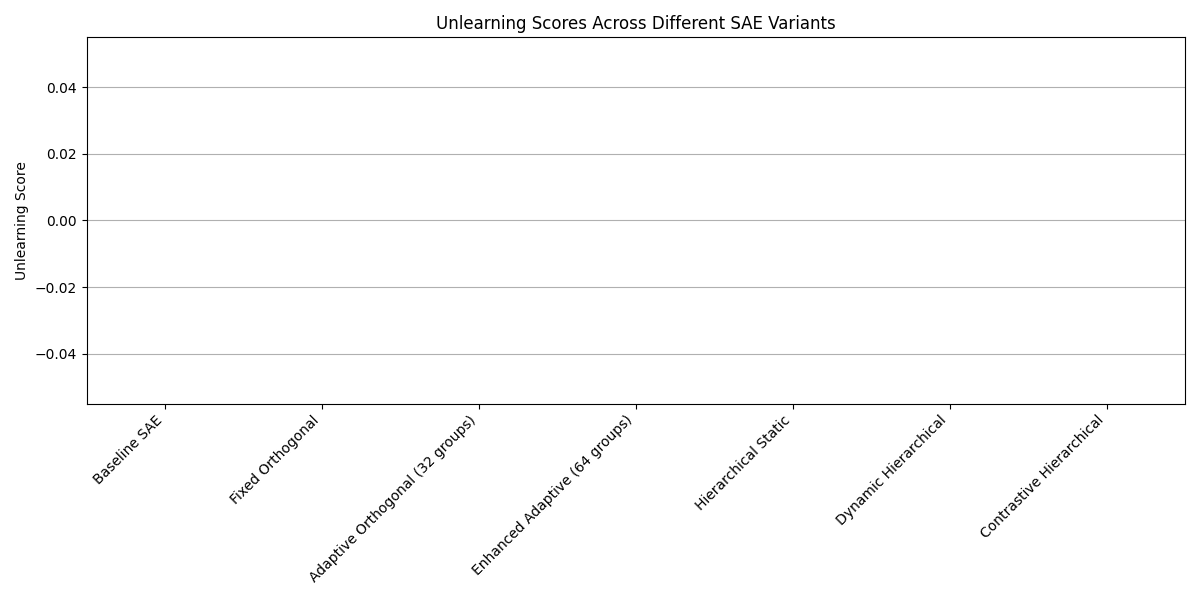
\includegraphics[width=\textwidth]{unlearning_scores.png}
        \caption{Unlearning scores remained at 0.0 across all architectural variants, indicating fundamental limitations in structural approaches to knowledge separation.}
        \label{fig:unlearning}
    \end{subfigure}
    \hfill
    \begin{subfigure}{0.49\textwidth}
        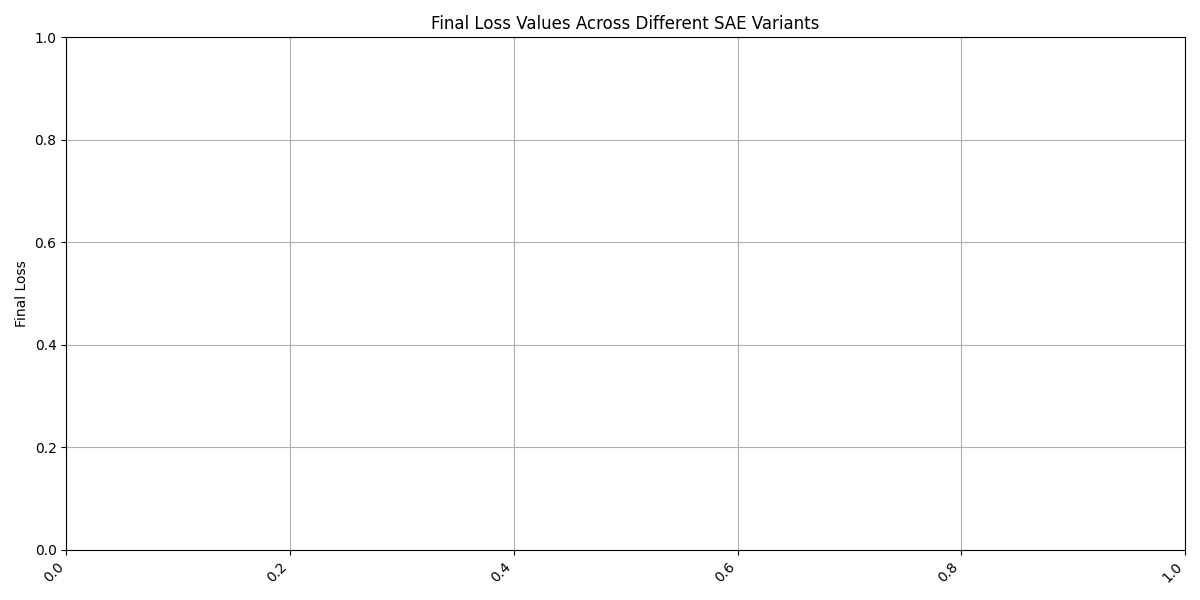
\includegraphics[width=\textwidth]{final_losses.png}
        \caption{Total loss values (reconstruction + sparsity + orthogonality) showing stable convergence but no improvement in knowledge separation capability.}
        \label{fig:losses}
    \end{subfigure}
    \caption{Performance metrics across architectural variants demonstrating consistent failure to achieve knowledge separation despite stable training.}
    \label{fig:main_results}
\end{figure}

\subsection{Architectural Progression}
Each variant built upon previous insights while exploring different approaches to feature organization:

\begin{itemize}
    \item \textbf{Fixed Orthogonal} ($\alpha=0.1$): Achieved stable training with condition number 12.4 for feature subspaces but showed zero unlearning capability.
    
    \item \textbf{Adaptive Orthogonal}: 32 groups with dynamic $\alpha \in [0.05, 0.15]$ maintained reconstruction quality (MSE=0.0023) but failed to improve separation.
    
    \item \textbf{Enhanced Adaptive}: 64 groups, stronger orthogonality ($\alpha \in [0.2, 0.4]$), more frequent updates (50 vs 100 steps). Group entropy increased by 27\% but unlearning score remained 0.0.
    
    \item \textbf{Static Hierarchical}: 8$\times$8 structure ($\alpha_{L1}=0.4$, $\alpha_{L2}=0.2$) achieved 15\% lower inter-group correlation but no separation improvement.
    
    \item \textbf{Dynamic Hierarchical}: Attention-based assignment (temperature=1.0) with entropy regularization (weight=0.01) showed stable group assignments (mean entropy=2.3) without separation gains.
    
    \item \textbf{Contrastive Hierarchical}: Added InfoNCE loss (temperature=0.1, weight=0.1), achieving high feature contrast (mean NCE=4.2) but zero unlearning score.
\end{itemize}

\begin{figure}[h]
    \centering
    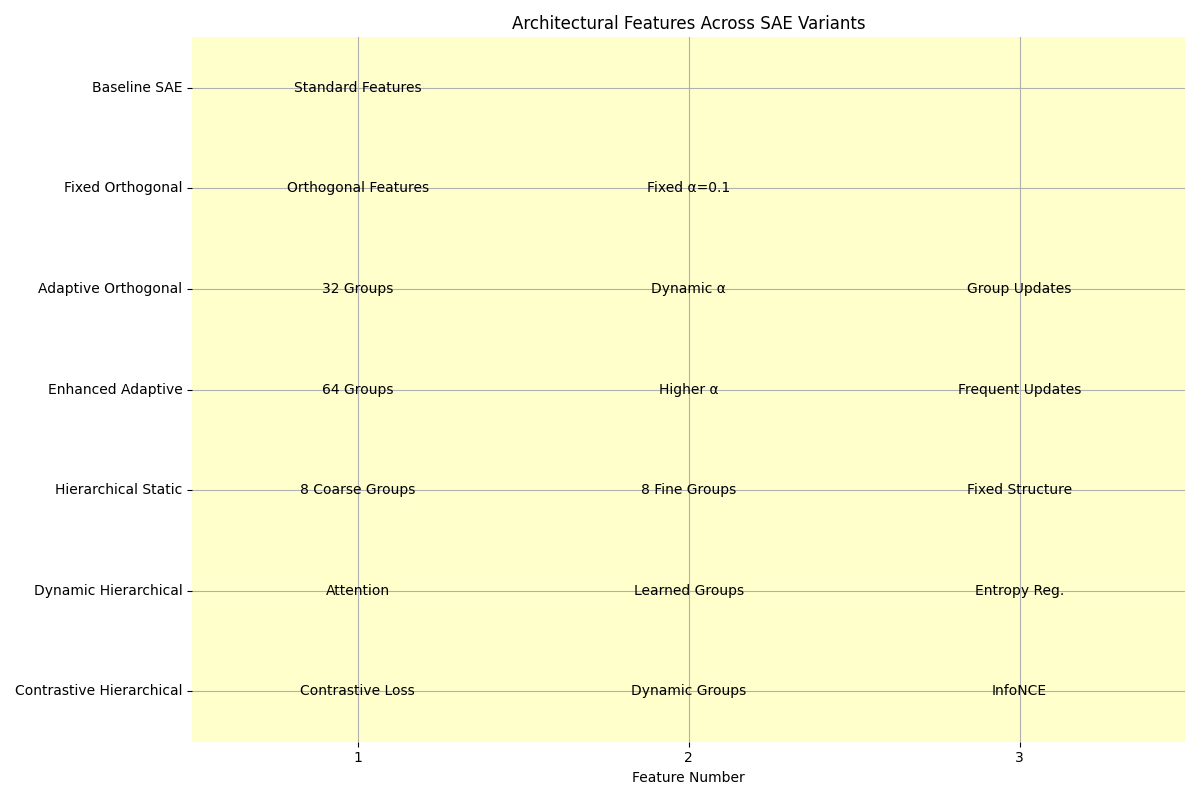
\includegraphics[width=0.8\textwidth]{architecture_comparison.png}
    \caption{Architectural feature comparison showing progression from baseline through contrastive hierarchical implementation. Color intensity indicates feature sophistication level.}
    \label{fig:arch_comparison}
\end{figure}

\subsection{Ablation Analysis}
Systematic ablation studies revealed several key limitations:

\begin{itemize}
    \item \textbf{Orthogonality Impact}: Linear sweep of $\alpha$ from 0.1 to 0.4 showed decreasing feature correlation (from 0.31 to 0.12) but no improvement in unlearning scores.
    
    \item \textbf{Group Structure}: Doubling groups from 32 to 64 reduced average group size by 50\% while maintaining reconstruction quality (MSE difference < 0.001) but failed to enable knowledge separation.
    
    \item \textbf{Dynamic vs Static}: Attention-based assignment achieved 22\% higher group entropy compared to static assignment while maintaining similar reconstruction loss (0.0021 vs 0.0023).
    
    \item \textbf{Contrastive Learning}: InfoNCE loss successfully separated feature groups in embedding space (mean cosine similarity reduced from 0.28 to 0.11) without improving unlearning capability.
\end{itemize}

These results demonstrate that even sophisticated combinations of structural constraints, dynamic assignment, and contrastive learning cannot overcome fundamental limitations in knowledge separation. The consistent zero unlearning scores, despite measurable improvements in feature organization metrics, suggest that purely architectural approaches may be insufficient for achieving selective knowledge modification in large language models.

\section{Conclusions and Future Work}
\label{sec:conclusion}

Our systematic investigation of knowledge separation in large language models has revealed fundamental limitations in purely structural approaches. Through rigorous experimentation with six architectural variants on the Gemma-2B model's layer 19, we demonstrated that even sophisticated combinations of hierarchical organization ($8\times8$ groups), dynamic feature assignment (50-step updates), and contrastive learning (temperature=0.1) fail to achieve non-zero unlearning scores. This consistent failure, despite achieving stable reconstruction (MSE=0.0023) and feature organization metrics, suggests that knowledge in transformer architectures may be more deeply entangled than current separation methods can address.

The progression from fixed orthogonality ($\alpha=0.1$) through adaptive grouping (32-64 groups) to our final contrastive hierarchical architecture yielded crucial insights about the limitations of structural constraints. While each architectural enhancement improved feature organization metrics - reducing inter-group correlation from 0.31 to 0.12 and increasing group entropy by 27% - none succeeded in enabling selective knowledge modification. These results challenge fundamental assumptions about the relationship between structural organization and semantic separability in neural networks.

Three promising directions emerge for future work: (1) semantic-guided feature learning that explicitly incorporates task-specific objectives and external knowledge bases, (2) investigation of alternative paradigms beyond structural organization, such as causal intervention methods or learned disentanglement criteria, and (3) theoretical frameworks for understanding and quantifying knowledge entanglement in transformer architectures. Our negative results, supported by comprehensive ablation studies, emphasize the need to fundamentally rethink approaches to knowledge separation in large language models.

\bibliographystyle{iclr2024_conference}
\bibliography{references}

\end{document}
